
% ****** Start of file apssamp.tex ******
%
%   This file is part of the APS files in the REVTeX 4.2 distribution.
%   Version 4.2a of REVTeX, December 2014
%
%   Copyright (c) 2014 The American Physical Society.
%
%   See the REVTeX 4 README file for restrictions and more information.
%
% TeX'ing this file requires that you have AMS-LaTeX 2.0 installed
% as well as the rest of the prerequisites for REVTeX 4.2
%
% See the REVTeX 4 README file
% It also requires running BibTeX. The commands are as follows:
%
%  1)  latex apssamp.tex
%  2)  bibtex apssamp
%  3)  latex apssamp.tex
%  4)  latex apssamp.tex
%
\documentclass[%
 reprint, linenumbers,
%superscriptaddress,
%groupedaddress,
%unsortedaddress,
%runinaddress,
%frontmatterverbose, 
%preprint,
%preprintnumbers,
%nofootinbib,
%nobibnotes,
%bibnotes,
 amsmath,amssymb,
 aps, physrev
%pra,
%prb,
%rmp,
%prstab,
%prstper,
%floatfix,
]{revtex4-2}

\usepackage{graphicx}% Include figure files
\usepackage{dcolumn}% Align table columns on decimal point
\usepackage{bm}% bold math
\usepackage{physics}
\usepackage{tikz}
\usetikzlibrary{arrows.meta, positioning}

%\usepackage{hyperref}% add hypertext capabilities
%\usepackage[mathlines]{lineno}% Enable numbering of text and display math
%\linenumbers\relax % Commence numbering lines

%\usepackage[showframe,%Uncomment any one of the following lines to test 
%%scale=0.7, marginratio={1:1, 2:3}, ignoreall,% default settings
%%text={7in,10in},centering,
%%margin=1.5in,
%%total={6.5in,8.75in}, top=1.2in, left=0.9in, includefoot,
%%height=10in,a5paper,hmargin={3cm,0.8in},
%]{geometry}

\begin{document}

\preprint{APS/123-QED}

\title{\textbf{The title should simply and concisely convey the main findings. Avoid nonstandard abbreviations and acronyms.} 
}% 


\author{Ann Author}
 \altaffiliation[Also at ]{Physics Department, XYZ University.}%Lines break automatically or can be forced with \\
\author{Second Author}%
 \email{Contact author: Second.Author@institution.edu}
\affiliation{%
 Authors' affiliations\\
  Include all institutions where the work was conducted: department or division, institution, city, state (if relevant), and country, in this order.
}%

\collaboration{CLEO Collaboration}%\noaffiliation

\date{\today}% It is always \today, today,
             %  but any date may be explicitly specified

\begin{abstract}
An article usually includes an abstract, a concise summary of the work
covered at length in the main body of the article. 
\end{abstract}

%\keywords{Suggested keywords}%Use showkeys class option if keyword
                              %display desired
\maketitle

%\tableofcontents

\section{\label{sec:level1}Theoretical framework}
In this section, the energy density funcitonal (EDF) employed is outlined.
\subsection{Skyrme EDF}
The total energy of the system can be expressed using an EDF by accounting for five different contributions:
\begin{align}
\label{eq:functional}
E&= E_\text{Kin} + E_\text{Sk} + E_\text{cm}+E_\text{Coul}+E_\text{Pair}\\
&= \int d\boldsymbol{r}[\mathcal E_\text{Kin} + \mathcal E_\text{Sk} + \mathcal E_\text{cm}+\mathcal E_\text{Coul}+\mathcal E_\text{Pair}],
\end{align}
where $E_\text{Kin}$ is the kinetic energy, $E_\text{Sk}$ the Skyrme energy, which models the strong interaction between the nucleons, $E_\text{cm}$ the center or mass correction, $E_\text{Coul}$ the electric repulsion due to the protons and $E_\text{Pair}$ the interaction describing pairing correlations.

\subsubsection{\label{sec:e_sk}Skyrme energy functional}
The Skyrme part of the EDF models the strong interaction between the nucleons. From this point forward we will restrict ourselves to the case of time-reversal symmetry of the nucleus. In such case, time-odd densities vanish, and the Skyrme energy reduces to~\cite{unedf, chabanat1, chabanat2}
\begin{eqnarray}
\nonumber
\mathcal E_\text{Sk} = \sum_{t=0,1}\bigg\{&C_t^{\rho}[\rho_0]\rho_t^2 +C_t^{\rho_t}\tau_t + C_t^{\Delta\rho}\rho_t\nabla^2\rho_t+\\\label{eq:skyrme}& +C_t^{\nabla\cdot \boldsymbol{J}}\rho_t\nabla\cdot\boldsymbol{J}_t + C_t^{\boldsymbol{J}^2}\boldsymbol{J}^2\bigg\},
\end{eqnarray}
where the index $t$ runs over $0$ for isoscalar densities and $1$ for isovector densities, respectively $\rho_0 = \rho_n + \rho_p$, $\rho_1 = \rho_n - \rho_p$ and similarly for all other quantities. $p$ and $n$ refer to protons and neutrons, respectively. The $C_t^\rho[\rho_0]$ coupling is further split into two contributions
\begin{equation}
  C_t^{\rho} = C_{t0}^\rho+C_{tD}^\rho \rho_0^\sigma.
\end{equation}
The different densities are defined starting from the density matrix in coordinate space 
\begin{equation}
  \rho_q(\bm r\sigma, \bm r'\sigma') = \expval{a_q^\dagger(\bm r\sigma)a_q(\bm r'\sigma')},
\end{equation}
where the index $\sigma=\pm 1$ runs over the up ($\sigma = 1$) and down ($\sigma = -1$) components of the spin.
The spin trace of the density matrix reads
\begin{align}
  \rho_q(\bm r, \bm r') = \sum_{\sigma =\pm 1}\rho_q(\bm r\sigma, \bm r'\sigma'),
\end{align}
and the spin density reads
\begin{equation}
  \bm s_q (\bm r, \bm r')=\sum_{\sigma\sigma' = \pm 1}\rho_q(\bm r, \bm r')\bra{\sigma'}\bm \sigma \ket{\sigma'},
\end{equation}
where $\bm \sigma$ is the vector of Pauli matrices.
The densities in Eq. \ref{eq:skyrme} are then defined as
\begin{align}
\rho_q &= \rho_q(\bm r, \bm r')|_{\bm r = \bm r'},
\\ \tau_q &= \nabla'\cdot\nabla\rho(\bm r, \bm r')|_{\bm r = \bm r'},
\\J_{q, \mu\nu} &= \frac{1}{2i}(\nabla_\mu - \nabla_\mu') s_{q, \nu}(\bm r, \bm r')|_{\bm r = \bm r'},
\\J_{q,\kappa}(\boldsymbol{r})&=\sum_{\mu\nu}\varepsilon_{\kappa\mu\nu}J_{q,\mu\nu}\label{eq:J_vec},
\end{align}
where $\varepsilon_{\kappa\mu\nu}$ is the Levi-Civita symbol.
The spin-orbit density current tensor $\bar{\bar J}$ contribution to the EDF is generally split into its irreducible components.
The scalar and tensor (irreps) parts vanish in our description, since they are time-odd \cite{conversions}. The only non-zero contribution is given by the time-odd vector component $J_{q,\kappa}$ defined in Eq. \ref{eq:J_vec}.
\subsubsection{Kinetic energy and center of mass correction}
The kinetic energy term reads
\begin{equation}
  \mathcal E_\text{Kin} = \frac{\hbar^2}{2m},
\end{equation}
while the loss of the center of mass symmetry loss is approximately compensated by the one-body center of mass correction correction term, which reads
\begin{equation}
  \mathcal E_\text{cm} = -\frac{1}{2mA}\sum_i \expval{p_i^2}.
\end{equation}
This equates to a renormalization of the nucleon mass, which then takes the form
\begin{equation}
  m\to m\frac{A}{A-1}.
\end{equation}
\subsubsection{Coulomb energy}
The Coulomb energy is treated within the Local Density Approximation. The resulting energy density reads~\cite{SlaterApp}
\begin{align}
    \mathcal E_\text{Coul} &=\mathcal E_{\text{Coul, D}}+\mathcal{E}_\text{Coul, E} \\&=\frac{e^2}{2}\bigg[\int  \frac{\rho_p(\bm r )\rho_p(\bm r ' )}{|\bm r-\bm r'|}d\bm r'  - \frac 3 2 \bigg(\frac 3 \pi \bigg) ^{\frac 1 3}\rho_p^{4/3}(\bm r)\bigg].\nonumber
\end{align}

\subsubsection{Pairing energy}
The pairing interaction is assumed to be different from the particle-hole one, as done extensively in the literature. Treating the particle-particle channel requires the definition of the skew-symmetric pairing tensor
\begin{equation}
\kappa_q (\bm r \sigma, \bm r'\sigma') = \expval{a_q(\bm r'\sigma') a_q(\bm r \sigma)},
\end{equation}
which can be casted on a pairing density matrix that reads
\begin{equation}
\tilde\rho_q(\bm r \sigma, \bm r'\sigma')=-2\sigma'\kappa_q(\bm r \sigma, \bm r'\sigma').
\end{equation}
The local pairing density finally reads 
\begin{equation}
  \label{eq:pairing_density}
\tilde\rho_q(\bm r)=\sum_{\sigma=\pm 1}\tilde\rho_q(\bm r \sigma, \bm r\sigma).
\end{equation}
In this work, we employ the zero-range interaction which results in the energy density~\cite{Bender2003}
\begin{equation}
    \mathcal E_\text{Pair} =\sum_{q=n,p} \frac 1 4 V_{q}\tilde\rho_q(\bm r)\tilde\rho_q^*(\bm r)\bigg[1-\eta\frac{\rho_0(\bm r)}{\rho_s}\bigg].
\end{equation}
Here, $\eta\in[0,1]$ is a parameter which controls the spatial strength of the pairing interaction, $\eta=0$ corresponds to volume pairing, $\eta=1$ to surface pairing, and mixed pairing otherwise. $\rho_s$ is the nuclear saturation density, fixed at $0.16$ fm$^{-3}$.
\subsection{HFB equations}
Minimizing the EDF constraining the single-particle wavefunctions orthonormality and the particle number leads to the Hartree--Fock--Bogoliubov equations
\begin{equation}
  \begin{pmatrix}
    h - \lambda & \Delta \\ -\Delta^* & -(h-\lambda)
  \end{pmatrix}
  \begin{pmatrix}
    U_\mu \\ V_\mu
  \end{pmatrix}
  =E_\mu \begin{pmatrix}
    U_\mu \\ V_\mu
  \end{pmatrix},
  \label{eq:HFB}
\end{equation}
where $E_\mu$ are the quasiparticle energies and $U_\mu$ and $V_\mu$ are the respective components of the quasiparticle wavefunctions. The mean-field Hamiltonian $h$ and the pairing field $\Delta$ are obtained as variations of the functional, respectively $h_{ij} = \delta \mathcal E / \delta \rho_{ij}$ and $\Delta_{ij} = \delta \mathcal E / \delta \kappa^*_{ij}$. 
$\lambda$ is a Langrange multiplier used to fix the particle number.

\subsubsection{Mean-field Hamiltonian}
The variation of the energy functional with respect to the density matrix $\rho_{ij}$ leads to the single-particle Hamiltonian, which projected on the coordinate basis reads
\begin{equation}
h=\nabla\cdot\frac{\hbar^2}{2m^*(\boldsymbol{r})}\nabla+U_{q}(\boldsymbol r)+B_q(\boldsymbol r)\cdot(\nabla\times\hat\sigma),
\end{equation}
where the different fields in the equation are computed from the variation of the energy functional with respect to the local densities
\begin{equation}
U_q = \frac{\delta \mathcal E}{\delta \rho},\ B_q = \frac{\delta \mathcal E}{\delta \boldsymbol{J}},\ m^*=\frac{\delta \mathcal E}{\delta \tau}.
\end{equation}
The self-consistent solution of Eq.~\ref{eq:HFB} in coordinate space can be obtained in different ways. In this work, we employ the two-basis method, a detailed discussion can be found in Refs.~\cite{cr8,TERASAKI19951,two_basis_hg_bands}.
\subsection{Two-basis method}
In the two-basis method, instead of diagonalizing the full HFB matrix, the problem is split into finding two bases: (a) the HF basis which diagonalizes the mean-field Hamiltonian $h$ and (b) the quasiparticle basis, expressed in the HF basis, which diagonalizes the HFB Hamiltonian.
In practice, this means that at each iteration, we solve the eigenvalue problem
\begin{equation}
  h\ket{\phi_k} = \varepsilon_k\ket{\phi_k},
\end{equation}
which yields the HF basis $\ket{\phi_k}$. We can then compute the local pairing density (Eq.~\ref{eq:pairing_density}) as 
\begin{equation}
  \tilde\rho_q(\bm r) = \sum_{\sigma=\pm 1}\kappa_{ij}f_i f_j\phi_i(\bm r\sigma)\phi_j(\bm r -\sigma),
\end{equation}
The pairing gaps in this basis are then computed as
\begin{equation}
\Delta_{ij}=\sum_{\sigma=\pm 1}\int d\bm r \frac{V_q} 2 \bigg[1-\eta\frac{\rho_0(\bm r )}{\rho_s}\bigg]\phi_i(\bm r \sigma)\phi_j(\bm r -\sigma)f_i f_j.
\end{equation}
The $f_i,f_j$ factors are used to regularize the pairing interaction, as $\mathcal E_\text{Pair}$ is local in the pairing density it implies constant coupling in momentum space. To avoid sudden changes in the states considered, the factors used are the ones proposed in Ref.~\cite{pairing_factors}, which read
\begin{equation}
  \nonumber
  f_i = \bigg[\frac 1 {1+e^{(\varepsilon_i-\lambda_q-\Delta\varepsilon_q)/\mu_q}}\cdot\frac 1 {1+e^{(-\varepsilon_i+\lambda_q-\Delta\varepsilon_q)/\mu_q}}\bigg]^{1/2},
\end{equation}
where $\Delta\varepsilon_q$ is the pairing window and $\mu_q$ is a factor which controls the sharpness of the window.
After diagonalizing the HFB Hamiltonian in this basis, the density matrix and the pairing tensor are computed as
\begin{equation}
\rho = V^*V^T,\quad \kappa = U^*V^T.
\end{equation}
The next mean field Hamiltonian is computed from the densities calculated on the canonical basis $\ket{\psi_i}$, i.e. the set of orbitals that diagonalizes the density matrix $\rho$
\begin{align}
 (S^{-1}\rho S)_{ij} =  \delta_{ij} v_i^2.
\end{align}
The canonical basis, in the HF basis thus reads
\begin{equation}
  \ket{\psi_i} = \sum_{k}S_{ki} \ket{\phi_k}.
\end{equation}

\subsection{The Lipkin-Nogami method}
The Lipking-Nogami method (LN)~\cite{Lipkin1960} is an approximate variation after projection of the particle number. In this framework the total energy of the system becomes
\begin{equation}
E[\rho, \kappa]\mapsto E[\rho, \kappa] -\lambda_2 (\expval{N^2}-\expval{N}^2).\label{eq:LN}
\end{equation}
The calculation of $\lambda_2$ is carried out at each iteration using the prescription~\cite{Stoitsov2007, Stoitsov2003}:
\begin{equation}
  \lambda_2=\frac{G_\text{eff}}{4}\frac{\Tr{(1-\rho)\kappa}\Tr{\rho\kappa}-2\Tr{(1-\rho)^2 \rho^2}}{[\Tr(1-\rho)]^2-2\Tr\rho^2(1-\rho)^2},
\end{equation}
where $G_\text{eff}$ is set to
\begin{equation}
  G_\text{eff}=-\frac{\bar\Delta^2}{E_\text{pair}}.
\end{equation}
Here, $\bar\Delta$ is the average pairing gap, computed as
\begin{equation}
  \bar\Delta = \frac{\Tr{\Delta\rho}}{\Tr\rho}.
\end{equation}
This phenomenological choice avoids the costly evaluation of the fields, which depends on the specific pairing interaction employed.
On top of an approximate particle projection (before variation), the Lipkin-Nogami method introduces a curvature in the energy surface which prevents pairing collapse. This is important in deformed calculations, as certain spatial configurations along iterations may result in the trivial solution $\Delta = 0$, which is not recoverable in an HFB calculation.
The substitution in~\eqref{eq:LN} modifies the HFB matrix~\eqref{eq:HFB}. Different choices can be made, depending on which expression for the particle dispersion is used~\cite{two_basis_hg_bands}. In this work, the choice 
\begin{equation}
  h\mapsto h-2\lambda_2(1-2\rho)
\end{equation}
is used.
\section{Numerical treatment}
\subsection{Numerical derivatives}
Derivatives at each iteration are computed using the lagrange mesh scheme~\cite{ryssens_precision}. This enables reaching very high accuracies even for very modest meshes and guarantees that the method is variational. The single-particle Hamiltonian $h$ is discretized with a five point scheme~\cite{finite_diff}.

\subsection{\label{sec:gcg}Implementation of the GCG method}
The minimization of the energy functional on a cartesian mesh by repeated diagonalization of the single-particle Hamiltonian $h$ is unfeasible. Even very modest discretizations lead to large-scale matrices which cannot be diagonlized exactly in reasonable CPU times. There exists a wide range of methods that can be employed for this kind of problem. One promising technique is the use of the preconditioned gradient descent~\cite{ryssens_numerical, covariant_lobpcg}. In this work we implement an algorithm based on the Generalized Conjugate Gradient (GCG) method~\cite{gcg1, gcg2}.

\subsubsection{Algorithm}
The method starts from a set of $N_b$ guess single-particle wavefunctions $\{\phi_k^{(0)}\}$ and iteratively updates them until some convergence criteria is satisfied.

At iteration $(i)$ of the procedure, a block $W$ is constructed by an application of the inverse single-particle hamiltonian $h^{(i)}$, approximately solving the linear system
\begin{equation}
    (h^{(i)}-\varepsilon_0^{(i)})W^{(i)}_k = \varepsilon^{(i)}_k\phi_k^{(i)},
\end{equation}
where $\varepsilon_0^{(i)}$ is the lowest single-particle energy at iteration $(i)$.
A conjugate search direction block is built using the previous iteration's states
\begin{equation}
P_k^{(i)} = \phi^{(i)}_k - \langle\phi_k^{(i-1)}| \phi_k^{(i)}\rangle\phi_k^{(i-1)}.
\end{equation}
The new states for the iteration $(i+1)$ are finally obtained by diagonalizing $h^{(i)}$ in the vector space
\begin{equation}\mathcal V^{(i)}=\text{span}\{W^{(i)}, P^{(i)}, F^{(i)}\}
\end{equation}
where $F^{(i)}$ is the block 
\begin{equation}
F_k^{(i)} = \phi_k^{(i)}.
\end{equation}
The diagonalization of $h^{(i)}$ in $\mathcal V^{(i)}$ is equivalent to solving the problem
\begin{equation}
  V^{(i)\dagger} h^{(i)} V^{(i)}C = \Lambda C
\end{equation}
which is of dimension $3N_b\times 3N_b$. $V^{(i)}$ is a matrix constructed by building the block $[W^{(i)}, P^{(i)}, F^{(i)}]$ and orthonormalizing it. $\Lambda$ is a diagonal matrix containing the eigenvalues of the small eigenvalue problem and $C$ is a matrix containing the eigenvectors.
The new eigenvectors $\{\phi_k^{(i+1)}\}$ are the ones corresponding to the lowest $N_b$ eigenvalues and they are obtained by
\begin{equation}
  \phi_k^{(i+1)} = \sum_{j=1}^{N_b} \phi_j^{(i)}C_{kj}.
\end{equation}

\subsubsection{Comparison with other algorithms}
As shown in Fig.~\ref{fig:conv_comp} GCG performs better when compared with the very similar counterpart LOBPCG~\cite{lobpcg}. It is not only faster, but more robust and stable as well, while maintaining an identical computational effort. Moreover, a filtering operator is not necessary when varitional collapse is a problem, e.g.~in the covariant case~\cite{covariant_lobpcg} or the self-consistent solution of the HFB matrix by minimization~\cite{hfb_ihm}. Additionally, no search for an optimal preconditioner is needed, as the single-particle matrix is used in the inverse step.

Another interesting comparison can be done with the Imaginary Time Evolution (ITE) method, used for example by the Skyrme code EV8~\cite{ev8}. While the computational overhead of ITE is very light, requiring only a matrix application and an orthonormalization of the eigenvectors, the execution time is dominated by the recalculation of the derivatives, blowing up the execution time: 159 s against the 21 s required by GCG.
\begin{figure}[ht]
  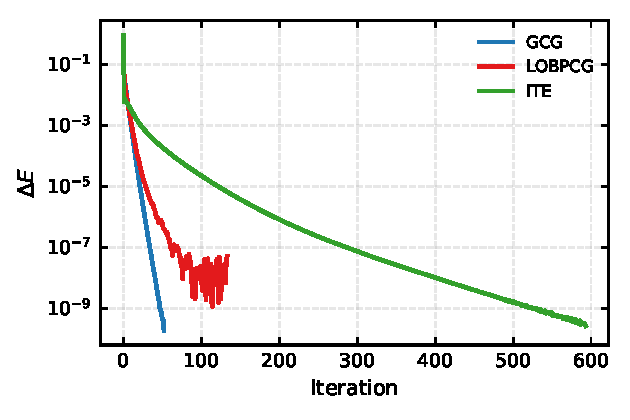
\includegraphics[ width=\columnwidth]{figures/conv_comp}
  \caption{Convergence of the total energy with three different algorithms. $^{40}$Ca using SLy5. $\Delta E^ { (i)} =| E^{(i)}-  E^{(i-1)}|/| E^{(i)}|$. }
  \label{fig:conv_comp}
\end{figure}

\subsection{\label{sec:alm}Spatial constraints}
Spatial constraints are implemented in this work by using the Augmented Lagrangian Method~\cite{ALM}, which minimizes the Routhian
\begin{equation}
E' = E + \lambda^{(i)} (\langle Q \rangle-q) + \frac c 2 (\langle Q\rangle -q)^2,
\end{equation}
where $Q$ is a multipole operator, $q$ a target value for said operator, and  $\lambda^{(i+1)}$ is a Lagrange multiplier updated at each mean field iteration using the damped scheme
\begin{equation}
    \lambda^{(i+1)} = \lambda^{(i)}+\mu c (\langle Q\rangle -q),
\end{equation}
where $\mu\approx 0.05$ is a constant used to damp oscillations of the constraint field~\cite{ev8}.

\subsection{Particle number constraint}
The lagrange multiplier $\lambda$ in~\eqref{eq:HFB} is used to fix the particle number average $\expval{N}$. It is determined during the diagonalization of the HFB matrix using a bisection algorithm.
This can be done by first determining a bracketing interval $[\lambda_\text{min}, \lambda_\text{max}]$ in which the correct value of $\lambda$ shall lie. The bisection algorithm then proceeds as follows:
(a) Diagonalize the HFB matrix 
\begin{equation}
\begin{pmatrix}
  h - \lambda^{(j)} & \Delta \\ -\Delta^* & -(h-\lambda^{(j)})
\end{pmatrix}
\begin{pmatrix}
  U_\mu \\ V_\mu
\end{pmatrix}^{(j)}
=E_\mu \begin{pmatrix}
  U_\mu \\ V_\mu
\end{pmatrix}^{(j)};
\end{equation}
(b) determine the particle number $\expval{N}^{(j)}$;
(c) if $\expval{N}^{(j)} < A$, set $\lambda_\text{min} = \lambda^{(j)}$; otherwise set $\lambda_\text{max} = \lambda^{(j)}$;
(d) set $\lambda^{(j+1)} = (\lambda_\text{min} + \lambda_\text{max})/2$. Repeat until convergence.

The superscript $(j)$ is used to avoid confusion between the outer mean-field iterations $(i)$ and the bisection iterations $(j)$. During the bisection algorithm, only the $\lambda^{(j)}$ value is updated, for which a new quasiparticle basis is obtained.

\appendix
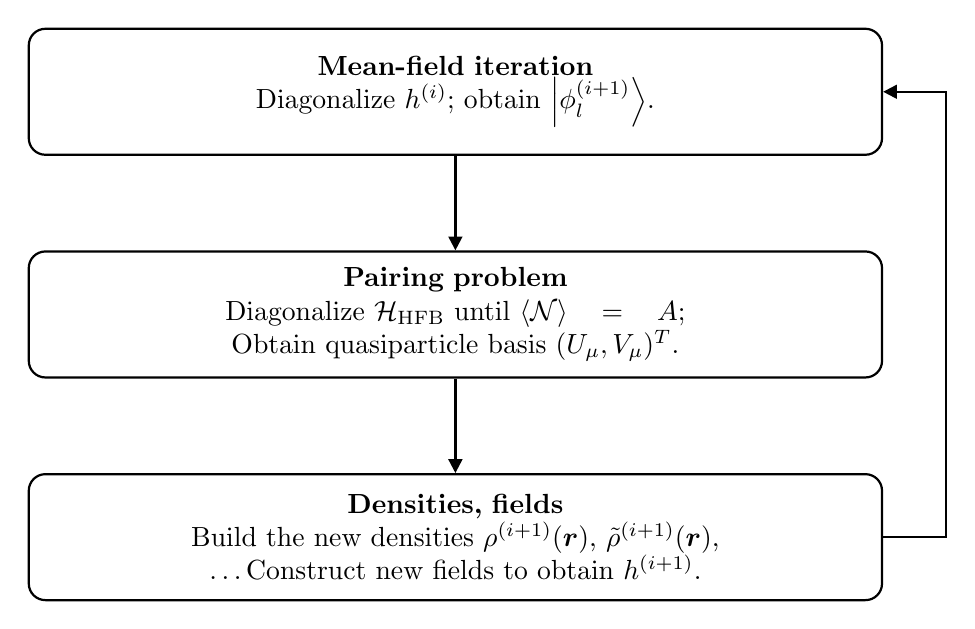
\begin{tikzpicture}[
    box/.style={
        draw,
        rounded corners=6pt,
        thick,
        align=center,
        text width=\linewidth-15mm,
        inner sep=3pt,
        minimum height=1.6cm
    },
    arrow/.style={
        -{Triangle[length=5pt,width=5pt]},
        thick
    }
]

\node[box] (diag) {
    \textbf{Mean-field iteration}\\
    Diagonalize ${h}^{(i)}$; obtain $\ket{\phi_l^{(i+1)}}$.
};

\node[box, below=1.2cm of diag] (pair) {
    \textbf{Pairing problem}\\
    Diagonalize $\mathcal H_\text{HFB}$ until $\langle\mathcal N\rangle=A$; Obtain quasiparticle basis $(U_\mu, V_\mu)^T$.
};

\node[box, below=1.2cm of pair] (scf) {
    \textbf{Densities, fields}\\
    Build the new densities $\rho^{(i+1)}(\bm r)$, $\tilde \rho^{(i+1)} (\bm r)$, \ldots Construct new fields to obtain $h^{(i+1)}$.
};

% vertical arrows
\draw[arrow] (diag) -- (pair);
\draw[arrow] (pair) -- (scf);

% compact feedback loop, fully inside column and centered
\draw[arrow]
    (scf.east) -- ++(8mm,0)
               |- (diag.east);

\end{tikzpicture}
\section{Local densities and fields}
We report here the formulae for the local densities in coordinate space
\begin{align}
    \rho_q(\boldsymbol{r}) =& \sum_{k,\sigma}v_k^2|\psi(\boldsymbol r \sigma)|^2,\\
    \tau_q (\boldsymbol{r})=& \sum_{k,\sigma} v_k^2 |\nabla\psi(\boldsymbol{r}\sigma)|^2,\\
    J_{q, \mu\nu} (\boldsymbol{r})=& \sum_{k,\sigma\sigma'} v_k^2\text{Im}\{{\psi(\boldsymbol{r}\sigma)\partial_\mu\sigma_{\nu,\sigma\sigma'}\psi(\boldsymbol{r}\sigma')}\},
    \\J_{q,\kappa}(\boldsymbol{r})=&\sum_{\mu\nu}\varepsilon_{\kappa\mu\nu}J_{q,\mu\nu}.
\end{align}
Here, the index $k$ runs over the canonical basis wavefunctions. $v_k^2$ denotes the occupation factor of the wavefunction $k$ computed by diagonalizing the density matrix.
\section{Mean-field}
The central field reads
\begin{align}
U_q =\;&
(2 C_{0}^{\rho} - 2 C_{1}^{\rho})\, \rho
+ 4 C_{1}^{\rho}\, \rho_q + \nonumber\\
& (C_{0}^{\tau} - C_{1}^{\tau})\, \tau
+ 2 C_{1}^{\tau}\, \tau_q + \nonumber\\
& (2 C_{0}^{\Delta\rho} - 2 C_{1}^{\Delta\rho})\, \nabla^2 \rho
+ 4 C_{1}^{\Delta\rho}\, \nabla^2 \rho_q + \nonumber\\
& (C_{0}^{\nabla J} - C_{1}^{\nabla J})\, \nabla \cdot \mathbf{J}
+ 2 C_{1}^{\nabla J}\, \nabla \cdot \mathbf{J}_q + \nonumber\\
& (\sigma+2)C_{0D}^\rho \rho^{\sigma+1}+\nonumber\\&C_{1D}^\rho\rho^{\sigma-1}(\sigma\rho_p^2+\sigma\rho_n^2+2\sigma\rho_p\rho_n + 2\rho_p^2-2\rho_n^2)\nonumber,
\end{align}
the spin-orbit field reads
\begin{align}
\bm B_q =& 2(C_0^{\bm J^2} - C_1^{\bm J^2})\bm J + 4C_1^{\bm J^2}\bm J_q - \nonumber\\
&(C_0^{\nabla \cdot \bm J} - C_1^{\nabla \cdot \bm J})\nabla \rho - 2C_1^{\nabla \cdot \bm J}\nabla \rho_q \nonumber,
\end{align}
and the effective mass field reads
\begin{align}
  \frac{\hbar^2}{2m^*}=&\frac{\hbar ^2}{2m}+\\
  &(C_0^\tau-C_1^\tau)\rho + 2C_1^\tau\rho_q + \nonumber\\
  &(C_0^\tau - C_1^\tau)\nabla \rho + 2C_1^\tau\nabla \rho_q. \nonumber
\end{align}
\subsection{Coulomb field}
The direct part of the Coulomb field, i.e.
\begin{equation}
  U_{c,D} = \frac{e^2}{2}\int d \bm r' \frac{\rho_p(\bm r')}{\|\bm r'-\bm r\|},
\end{equation}
is computed by solving the Poisson equation
\begin{equation}
  \nabla^2 U_{c, D} = -4\pi e^2\rho_p
\end{equation}
to avoid the costly evaluation of the integral. The energy density is then set to
\begin{equation}
  \mathcal E_\text{Coul, D} = U_{c,D}\rho_p.
\end{equation}
The exchange field reads
\begin{equation}
  U_{c, E} = \fdv{\mathcal E_\text{Coul, E}}{\rho} = -e^2\bigg(\frac 3 \pi \bigg)^{1/3}\rho_p^{1/3}.
\end{equation}
\subsection{Constraint field}
If constraints are present, the constraint field reads
\begin{equation}
  U_\text{Constr} = \lambda^{(i)} Q + c(\expval Q-q)Q.
\end{equation}
\newpage

%\section{Energy calculation}
%The nucleus energy can be computed in two ways. The trivial way is to evaluate the functional
%\begin{equation}
%  E = E[\rho, \tau, \bar{\bar J}].
%\end{equation}
%A different approach is to derive an expression from the single-particle Hamiltonian. On an arbitrary basis, the energy reads
%\begin{equation}
%  E = \Tr{\rho t} + \frac{1}{2}\Tr{\Tr{\rho \bar v[\rho]\rho}} + \frac{1}{4}\Tr{\Tr{\kappa^\dagger \bar v[\rho_0] \kappa}},
%\end{equation}
%where $\Tr{a}$ denotes the trace of the matrix $a$. The variation of the energy with respect to the density matrix and the pairing tensor read
%\begin{align}
%  h=&\fdv{E}{\rho} \\=& t + \Tr{\bar v [\rho_0] \rho} +\\&+ \frac 1 2 \Tr{\rho \fdv{\bar v[\rho]}{\rho}\rho}+\frac 1 4 \Tr{\kappa^\dagger \fdv{\bar v[\rho]}{\rho}\kappa}\nonumber,
%  \\\Delta =& \fdv{E}{\kappa^*}=\frac 1 4 \Tr{\bar v[\rho]\kappa}\nonumber.
%\end{align}
%From these two variations, the total energy can be recovered as
%\begin{equation}
%  E = \Tr{\rho  h} - \frac 1 2 \Tr{\rho \bar v[\rho]\rho} + \frac{1}{4}\Tr{\kappa^\dagger \Delta} + E_\text{rea},
%\end{equation}
%where $E_\text{rea}$ is the rearrangement energy, which is needed to account for the dependence of the interaction on the density and make the two expressions equivalent.
%At convergence, we have that $h\phi_k = \varepsilon_k\phi_k$, 


\nocite{*}

\bibliography{bibliography}

\end{document}
%
% ****** End of file apssamp.tex ******


